\documentclass[a4paper]{ctexrep}
\usepackage[colorlinks,linkcolor=black]{hyperref}
\usepackage{listings, geometry, amsmath}
\usepackage[colorinlistoftodos]{todonotes}
\usepackage{graphicx}
%\setmonofont[Mapping={}]{Monaco}	%英文引号之类的正常显示,相当于设置英文字体
\definecolor{mygreen}{rgb}{0,0.6,0}
\definecolor{mygray}{rgb}{0.5,0.5,0.5}
\definecolor{mymauve}{rgb}{0.58,0,0.82}
% 代码块设置
\lstset{ % 代码高亮
	backgroundcolor=\color{white},   % choose the background color
	basicstyle=\footnotesize\ttfamily,        % size of fonts used for the code
	columns=fullflexible,
	numbers=left,                    % where to put the line-numbers; possible values are (none, left, right)
	numbersep=0.5em,		% how far the line-numbers are from the code
	breaklines=true,                 % automatic line breaking only at whitespace
	captionpos=t,                    % sets the caption-position to bottom
	tabsize=4,
	frame = single,
	framexleftmargin=2em,
	commentstyle=\color{mygreen},    % comment style
	escapeinside={\%*}{*)},          % if you want to add LaTeX within your code
	keywordstyle=\color{blue},       % keyword style
	stringstyle=\color{mymauve}\ttfamily,     % string literal style
	rulecolor=\color{black},
	% identifierstyle=\color{red},
	language=c++,
	showtabs = false,
	showstringspaces = false,
	showspaces = false,
}

\geometry{left=3cm,right=3cm,top=3cm,bottom=3cm}

\hypersetup{
	pdftitle={实验报告模板},
	pdfauthor={刘朝洋},
	pdfsubject={实验报告模版},
	pdfkeywords={模版},
}

\ctexset {
	chapter = {
		name = {实验, },
	},
	section = {
		number = \arabic{section},
		format = \Large\bfseries,
	},
	subsection = {
		number = \arabic{section}.\arabic{subsection},
	}
}

\begin{document}
	\begin{titlepage} % 封面
		\begin{center}
		
\includegraphics[width=12cm]{img/cover3.jpg}\\[1cm]
		{\zihao{2} \kaishu \textbf{信息工程学院}\\[0.5cm]
		\textbf{实验报告}\\[3cm]}
		
		\vspace*{\fill}
		\begin{tabular}{l}
			\zihao{3}\songti
			实验名称: 图像增强\\[0.5cm]\zihao{3}\songti
			专业班级: 计算机141\\[0.5cm]\zihao{3}\songti
			学号: 2014012537\\[0.5cm]\zihao{3}\songti
			姓名: 刘朝洋\\[0.5cm]\zihao{3}\songti
			指导教师: 杨龙\\[0.5cm]\zihao{3}\songti
		\end{tabular}

		\vspace*{\fill}
		{\zihao{3} \songti 2016\textasciitilde 2017学年第一学期}\\[0.5cm]
		{\zihao{4} \songti 使用\LaTeX 撰写于\today}
		\end{center}
	\end{titlepage}
\tableofcontents % 目录
\chapter{图像平滑:以中值滤波为例}
\section{实验目的}

\begin{enumerate}
\item 掌握图像平滑的基本概念,以及常用的方法;
\item 了解不同滤波方法的原理,并可以编程实现。
\end{enumerate}
\section{实验要求}
\begin{enumerate}
\item 使用C++编程实现中值滤波,但不能直接调用OpenCV中的滤波函数;
\item 将处理结果与OpenCV中的平滑处理函数\lstinline|medianBlur()|的处理结果做对比。
\end{enumerate}

\section{实验过程}

中值滤波的原理很简单,它把以某像素为中心的小窗口内的所有像素的灰度按从小到大排序,取排序结果的中间值作为该像素的灰度值。

首先是放置窗口,这里我们通过改变开始的索引值来放置窗口。

\begin{lstlisting}
for (int m = 1; m < M - 1; ++m)
		for (int n = 1; n < N - 1; ++n)
\end{lstlisting}

注意,这里是从第1个元素开始,而不是第0个元素;倒数第1个元素结束,而不是最后一个元素。问题就是我们无法从第0个元素开始,因为在这种情况下,过滤窗口的左半部分是空的。为了解决这个问题,我们需要在处理之前,对图像的进行扩展,方法如下图\ref {fig:imgExt}所示:
\begin{figure}
\centering
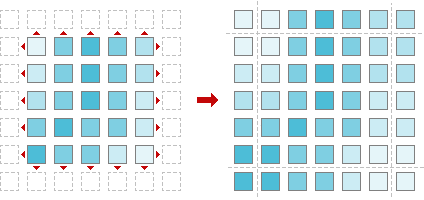
\includegraphics{img/extendImg.png}
\caption{图像扩展}
\label{fig:imgExt}
\end{figure}

\begin{lstlisting}
void medianfilter(element* image, element* result, int N, int M)
{
	//   Check arguments
	if (!image || N < 1 || M < 1)
		return;
	//   Allocate memory for signal extension
	element* extension = new element[(N + 2) * (M + 2)];
	//   Check memory allocation
	if (!extension)
		return;
	//   Create image extension
	for (int i = 0; i < M; ++i)
	{
		memcpy(extension + (N + 2) * (i + 1) + 1, image + N * i, N * sizeof(element));
		extension[(N + 2) * (i + 1)] = image[N * i];
		extension[(N + 2) * (i + 2) - 1] = image[N * (i + 1) - 1];
	}
	//   Fill first line of image extension
	memcpy(extension, extension + N + 2, (N + 2) * sizeof(element));
	//   Fill last line of image extension
	memcpy(extension + (N + 2) * (M + 1), extension + (N + 2) * M, (N + 2) * sizeof(element));
	//   Call median filter implementation
	_medianfilter(extension, result ? result : image, N + 2, M + 2);
	//   Free memory
	delete[] extension;
}
\end{lstlisting}
\section{实验总结}

\end{document}
